\part{Calcolo delle Variazioni}

\section{Preliminari}
Il calcolo delle variazioni si occupa dell'ottimizzazione di funzioni $\realfunction{F}{X}{\mathbb{R}}$, dove $X$ è un insieme di funzioni.\\
In questo capitolo varranno considerati univocamente funzionali integrali del tipo
$$\begin{array}{rcl} F: X & \to & \mathbb{R} \\
x & \to & \int_{a}^b f(t,x(t), x'(t))\integrald{t}\end{array}$$
eventualmente soggetti a vincoli sui valori $x(a)$ e $x(b)$ o sul valore di un integrale del tipo $\int_a^b \varphi(x(t))\integrald{t}$.\\
Dove:
$$\realfunction{f}{\realintervalclose{a}{b}\times\mathbb{R}^n\times\mathbb{R}^n}{\mathbb{R}}$$
$$X=\left\{x\in \cntclass{1}(\realintervalclose{a}{b});\mathbb{R}^n\text{ t.c.: }x(a)=x_a, x(b)=x_b \right\},\text{ con }x_a,x_b\in\mathbb{R}^n$$
\proposition
Sia $f\in \cntclass{1}(A\times\mathbb{R};\mathbb{R})$ con $a\subseteq\mathbb{R}^n$\\
Se $\begin{array}{ccc} F: \mathbb{R}\times\mathbb{R}\times A & \to & \mathbb{R} \\
x & \to & \int_{\alpha}^\beta f(x,t)\integrald{t}\end{array}$
Allora:
$$ F\in \cntclass{1}$$
$$ \partial_\alpha F(\alpha,\beta,x)=-f(x,\alpha)$$
$$ \partial_\beta F(\alpha,\beta,x)=f(x,\beta)$$
$$ \nabla_x F(\alpha,\beta,x)=\int_{\alpha}^{\beta}\nabla_xf(x,t)\integrald{t}$$
\definition ?????????????? R OPPURE RN\\
Sia $I\in\mathbb{R}$ un intervallo. Curva su $I$ $\mathbb{R}\rightleftharpoons$ una funzione $\gamma:I\subseteq\mathbb{R}^n$ che sia continua.
\observation
$\gamma(I)$ si chiama supporto della curva,ed 1'e certamente connesso.(una funzione continua manda intervalli connessi in connessi)
\definition
Sia $\realfunction{\gamma}{\realintervalclose{a}{b}}{\mathbb{R}}^n$ una curva, lunghezza della curva $\rightleftharpoons l(\gamma)=\sup\left\{\sum\limits_{i=1}^{N}\norm{\gamma(t_i)-\gamma(t_{i-1})}: N\in\mathbb{N}\,N>1,t_0=a,t_N=b,t_{i-1}<t_i, i=1,2,\ldots,N \right\}$ 
cioè prendo una curva e la approssimo con una spezzata, la più lunga di tutte le poligonali è la lunghezza della curva.\\
DISEGNO\\
DISEGNO\\
\definition
Una curva $\realfunction{\gamma}{\realintervalclose{a}{b}}{\mathbb{R}^n}$ si dice rettificabile $\rightleftharpoons f(\gamma)<+\infty$
\observation
$$\sum\limits_{i=1}^{N}\norm{\gamma(t_i)-\gamma(t_{i-1})} $$
per il teorema del valore medio differenziale(accrescimenti finiti)
$$\sum\limits_{i=1}^{N}\norm{ \gamma'(t_i)(t_i-t_{i-1})} =??$$
$$\int_{a}^{b}\norm{ \gamma'(t)} \integrald{t}$$
\proposition
Se $\gamma\in \cntclass{1}(\realintervalclose{a}{b};\mathbb{R}^n)\Rightarrow l(\gamma)=\int_a^b\norm{\gamma'(t)}\integrald{t}$
\observation
Se $\gamma$ è la traiettoria di un punto materiale,allora $\norm{\gamma}$ è la norma della velocità istantanea, e quindi $l(\gamma)$ è lo spazio che si percorre, cioè l'integrale della velocità valutato tra $t??????t_i$ due istanti di tempo entro i quali si mantiene tale velocità.
\observation
Nel caso specifico sarà:
$$ X=\left\{ x\in \cntclass{1}(\left[a,b\right];\mathbb{R}2): x(a)=A, x(b)=B \right\} $$
$$\begin{array}{ccc} 
F: X & \to & \mathbb{R} \\
x & \to & \int_{a}^b \norm{x'(t)}\integrald{t}
\end{array}$$
$$\begin{array}{ccc} 
f: \left[a,b\right]\times\mathbb{R}^2\times\mathbb{R}^2 & \to & \mathbb{R} \\
(t,x, x') & \to &  \norm{x'(t)}
\end{array}$$
\section{L'Equazione di Eulero}
LEMMA:::LEMMA FONDAMENTALE DEL CALCOLO DELLE VARIAZIONI\\
Sia $f\in \cntclass{0}(\left[0,1\right];\mathbb{R})$ t.c.: $\forall v\in \cntclass{0}(\left[0,1\right];\mathbb{R})$ con $v(0)=v(1)=0$ si abbia $\int_0^1 f(x)v(x)\integrald{x}=0$\\
Allora $f(x)\equiv 0\forall x\in\left[0,1\right]$ 
\begin{proof}
	\begin{center}
		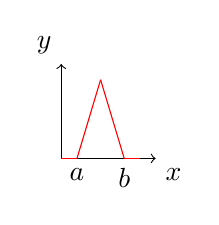
\begin{tikzpicture}[scale=1]
			\draw[->] (0,0) -- (1.2,0) node[anchor=north west] {$x$};
			\draw[->] (0,0) -- (0,1.2) node[anchor=south east] {$y$};
			\node[below] at (0.2,0) {$a$};
			\node[below] at (0.8,0) {$b$};
			\clip (0,0) rectangle (1,1);
			\draw[domain=0:0.2,smooth,red,variable=\x] plot ({\x},{0});
			\draw[domain=0.2:0.5,smooth,red,variable=\x] plot ({\x},{(1/0.3)*\x-(0.2/0.3)});
			\draw[domain=0.5:0.8,smooth,red,variable=\x] plot ({\x},{-(1/0.3)*\x+(0.8/0.3)});
			\draw[domain=0.8:1,smooth,red,variable=\x] plot ({\x},{0});
		\end{tikzpicture}
	\end{center}
	Per Assurdo, se $f\not\equiv 0$, allora $\exists\left[0,1\right]$ t.c. $f(x_0)\ne 0$.\\
	Osservo che se $x_0=0$ allora $\exists\overline{x}_0\in\left]0,1\right[$ t.c. $f(\overline{x}_0)\ne 0$.\\
	Osservo che se $x_0=1$ allora $\exists\overline{x}_0\in\left]0,1\right[$ t.c. $f(\overline{x}_0)\ne 0$\\
	Entrambe le osservazioni per la continuità di $f$, significa che se $x_0$ è un punto in cui la $f>0$ allora per la continuità della funzione anche li vicino si hanno valori maggiori di zero.\\
	Quindi si può pensare $x_0\in\left]0,1\right[$.\\
	Allora $\exists a,b\in\left]0,1\right[$ t.c. $x_0\in\left]a,b\right[ e \forall x\in\left]a,b\right[$ vale che $\abs{f(x)}\ge\abs{f(x_0)}$ sempre per la continuità di $f$.\\
	Pensiamo $f(x_0)>0$ in questo modo $\abs{f(x_0)}=f(x_0)$ e scegliamo la funzione $v(x)$ come disegnata: $v(x)=\left\{\begin{matrix}
	0&&x\le x_0-\delta\\
	\frac{x}{\delta}-\frac{x_0-\delta}{\delta}&& x_0-\delta<x<x_0\\
	1&& x=x_0\\
	-\frac{x}{\delta}+\frac{x_0+\delta}{\delta}&&x_0<x<x_0+\delta\\
	0&&x\ge x_0+\delta
	\end{matrix}\right.$POSSIBILIPLAUSIBILIERRORI\\
	Se calcoliamo
	$$\int_0^1f(x)v(x)\integrald{x}=\int_a^bf(x)v(x)\integrald{x}\ge\frac{1}{2}f(x_0)\int_a^bv(x)\integrald{x}=\frac{1}{2}f(x_0)\frac{b-a}{2}>0$$
	Se avessi preso $f(x_0)<0$ prendo $v=-v$ e il resto segue...
\end{proof}
\observation
Questo lemma è concettualmente analogo al Teorema di Fermat nel capitolo delle derivate.
\corollary LEMMA CASO VETTORIALE.\\
Sia $f\in \cntclass{0}(\left[a,b\right];\mathbb{R}^n)$ tale che $\forall v\in \cntclass{0}(\left[a,b\right];\mathbb{R}^n)$ con $v(0)=v(1)=0$ si abbia $\int_0^1f(x)\bullet v(x)\integrald{x}=0$ allora $f(x)\equiv 0$ $\forall x\in \left[0,1\right]$.
\begin{proof}
	Per questa dimostrazione si osservano componente per componente.\\
	$\forall i=1,2,\ldots,n$ scelgo $v_j(x)=\left\{\begin{matrix}0&&j\ne i\\v_i(x)&&j=i \end{matrix}\right.$\\
	A questo punto applico il lemma fondamentale alla componente $i$-esima $f_i$ di $f$.
\end{proof}
\corollary
Sia $f\in \cntclass{0}(\left[a,b\right];\mathbb{R})$ e $k\in\mathbb{N}$ tale che $\forall v\in \cntclass{k}(\left[a,b\right];\mathbb{R}^n)$ con $v(0)=v(1)=0$ si abbia $\int_0^1f(x)v(x)\integrald{x}=0$ allora $f(x)\equiv 0$ $\forall x\in \left[0,1\right]$.
\begin{proof}
	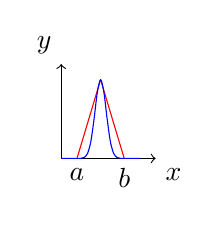
\begin{tikzpicture}[scale=1]
		\draw[->] (0,0) -- (1.2,0) node[anchor=north west] {$x$};
		\draw[->] (0,0) -- (0,1.2) node[anchor=south east] {$y$};
		\node[below] at (0.2,0) {$a$};
		\node[below] at (0.8,0) {$b$};
		\clip (0,0) rectangle (1,1);
		\draw[domain=0:0.2,smooth,red,variable=\x] plot ({\x},{0});
		\draw[domain=0.2:0.5,smooth,red,variable=\x] plot ({\x},{(1/0.3)*\x-(0.2/0.3)});
		\draw[domain=0.5:0.8,smooth,red,variable=\x] plot ({\x},{-(1/0.3)*\x+(0.8/0.3)});
		\draw[domain=0.8:1,smooth,red,variable=\x] plot ({\x},{0});
		\draw[domain=0:1,smooth,blue,variable=\x] plot ({\x},{ e^(-((\x-0.5)*10)^2) });
	\end{tikzpicture}
	\'E sempre lo stesso lemma con l'aggiunta che la funzione $v$ sia di classe $\cntclass{k}$.\\
	Se si chiama $u$ la funzione blu e $v$ la funzione rossa abbiamo:
	$$\int_0^1 f(x)u(x)\integrald{x}>0$$
	Se $v$ è un po più regolare , prendiamo $v=u^(k+1)(x)$. cioè se vogliamo $v\in \cntclass{k}$ prendiamo.....\\
	LA DINMOSTRAZIONE E A ME INCOMPRENSIBILE.
\end{proof}

\theorem EQUAZIONE DI EULERO.\\
Sia $f\in \cntclass{2}\left(\left[a,b\right]\times\mathbb{R}^n\times\mathbb{R}^n;\mathbb{R}\right)$ con $a,b\in\mathbb{R}$ e $a<b$.\\
Sia $X=\left\{x\in \cntclass{2}\left(\left[a,b\right];\mathbb{R}^n\right): x(a)=A, x(b)=B\right\}$ con $A,B\in\mathbb{R}^n$.\\
Sia $\begin{array}{ccc} F: X & \to & \mathbb{R} \\
x & \to & \int_{a}^b f(t,x(t), x'(t))\integrald{t}\end{array}$.\\
Se la funzione $x_\ast\in X$ è t.c. $F(x_\ast)=\max\left\{F(x):x\in X \right\}$ [o min]\\
Allora $\partial_xf(t,x_\ast(t), x_\ast'(t))-\frac{d}{\integrald{t}}\partial_{ x'}f(t,x_\ast(t), x_\ast'(t))=0$.\\
Questa ultima equzione è l'equazione di Eulero-Lagrange del Funzionale $F$ o a volte detta variazione prima del funzionale $F$. è un sistema di $n$ equazioni differenziali ordinarie del secondo ordine nella funzione incognita $x_\ast$.
\begin{proof}
	 Sia $\varphi(h)=F(x_\ast+hv)$, dove $x_\ast\in X$ e $x_\ast+hv\in X$, con $h$ piccolo.\\
	 L'equazione di Eulero-Lagrange in apparenza complicata è analoga ad un equazione di analisi1 del tipo $f'=0$ oppure in analisi due a $\nabla f=0$. solo che ora sono cavoli amari.\\
	 Come si sceglie la variazione $v$ in modo che $x_\ast+hv\in X$, con $h$ piccolo.\\
	 $X$ è l'insieme delle funzioni di $\cntclass{2}$, si sa che $x_\ast\in \cntclass{2}$, una scelta opportuna di $v$ è $v\in \cntclass{2}(\left]a,b\right[;\mathbb{R}^n)$.\\
	 Inotre deve essere che $ x_\ast(a)+hv(a)=A$ e  $x_\ast(b)+hv(b)=B$ per restare dentro l'insieme $X$.
	 Quindi $v(a)=v(b)=0$.
	 $h$ è uno scalare e per ipotesi si sa che $F(x_\ast)$ è punto di massimo, quindi si conclude che $h=0$ è punto di massimo per la funzione $\varphi$.\\
	 ........ 
\end{proof}
e qui finiscono gli appunti almeno per conto mio.


